\chapter{面向隐私保护的风险自适应访问控制模型}
\label{chap:RaBAC-for-privacy}

\section{引言}
\label{sec:intro}
随着云计算的发展和模型的广泛采用,云越来越多地存储和处理敏感数据和隐私信息,因此云面临着一些安全问题。身份和访问管理对于确保云中数据的隐私,机密性和完整性等特性至关重要。尽管访问控制对云安全非常有帮助,但是在云中最广泛实现的传统访问控制模型仍然存在问题。传统访问控制模型,例如ACL (访问控制列表) \cite{qian2001acla}, RBAC (基于角色的访问控制) \cite{jung2012cribac}, ABAC (基于属性的访问控制) \cite{zhang2011attribute} and PBAC (基于策略的访问控制) \cite{huang2011policy} 是严格和静态模型, 管理员预定义的所有访问策略。 在像云环境这样的“需要共享”的大规模信息系统中,用户和资源都是动态的并且一直在变化,不可能预先定义访问策略,而传统的访问控制方法也适合这种情况。

为了解决此问题,已经引入了基于风险的访问控制\cite{ni2010risk,shaikh2012dynamic,wang2011quantified,choi2015framework} 因为它们将风险级别分析作为授权决策过程的主要输入。 基于风险的访问控制通过考虑访问请求的环境和情况以及安全策略来评估风险,并根据阈值确定访问权限。这种决定访问权限的方式可以通过反映情况的本质并防止由于内部人员滥用和滥用数据而导致不必要的信息访问和泄漏,从而实现动态访问控制 \cite{chen2011risk}. 因此,风险量化成为基于风险的访问控制中的核心组件。传统上,风险定义为资源的潜在损失值。并且在信息系统中,访问风险可以被视为访问所揭示信息的潜在价值。以基于风险的访问控制为中心的现有工作提供了不同的方法来确保访问对象的安全性和私密性。 Chen等。 \cite{cheng2007fuzzy} 提出了一种模糊多级风险访问模型,该模型采用模糊理论来评估对象的通行等级和对象敏感度等级对, Ni等人\cite{ni2010risk} 将此思想扩展为基于该方法的模糊推理。Wang和Jin\cite{wang2011quantified} 在健康信息系统的访问控制中提出了一种基于条件熵的风险量化方法,以保护患者的隐私。Shaikh等。 提出了一种基于动态风险的访问控制系统决策方法的新方法,同时考虑了近代历史和悠久历史。Khambhammettu等\cite{khambhammettu2013framework} 提出了一种基于动态风险的访问控制系统决策方法的新方法,同时考虑了近代历史和悠久历史。Choi等\cite{choi2015framework} 对上下文信息进行了分类,通过扩展可扩展的访问控制标记语言 (XACML) 来应用风险,从而通过基于上下文和处理的权限配置文件和规范来估计和应用风险。但是所有这些工作都需要使用相同的方法来对访问对象 (用户) 和访问主题 (资源或信息)进行分类, 并且在特定情况下很难找到这种方法。 尽管现有工作可以动态地基于风险来决定许可,但是最大可容忍风险值 (风险阈值) 是静态的,且对于所有用户而言都是相同的,并且始终缺乏激励机制。

我们的目的是弥合上述差距。本文提出了一种基于马尔可夫和信息论的云大数据风险自适应访问控制模型。首先,为基于风险的访问控制模型定义了一个对手模型,提出了一些自然而有用的假设和定义。我们仅通过比较访问行为模式就为访问请求和用户提供了正式的分类模型。然后,提出了一种基于XACML的风险自适应访问控制框架。在此框架中,添加了三个新组件(策略风险评估点 (PREP), 会话控制和风险缓解服务) 并增强了三个标准组件 (策略执行点,策略访问点和策略信息点) 对于PREP,设计了一些明确的公式和方法,以根据过去的访问行为来计算访问请求的风险值,基于请求标识来允许访问请求,并根据访问历史定期计算用户风险,并设计激励机制通过重新定位风险配额和消耗风险配额。所有这些公式和方法都是准马尔可夫模型。

本文主要由如下组织构成。 在 \ref{sec:relate}部分介绍了与我们的方法相关的现有工作;  在 \ref{sec:adversary_model}部分中,介绍了一个对手模型和一些基于风险的访问控制模型的有用定义; 然后在\ref{sec:proposed model}部分中介绍基于XACML的框架和访问模型的细节,在 \ref{sec:Discussion and analysis}部分中将进行讨论和分析。 最后,我们完成了这项工作。

\section{相关工作}
\label{sec:relate}
以风险为中心的访问控制模型最近吸引了研究人员的注意 \cite{wang2011quantified,shaikh2012dynamic,choi2015framework}。Wang和Jin\cite{wang2011quantified} 考虑了一种实际的访问控制模型,该模型通过考虑医疗保健的实际情况来保护电子医疗系统中的患者隐私。首先,该模型允许医生通过量化与医生的数据访问活动相关的风险来做出访问决策。其次,该模型利用医生的整体统计行为和Shannon条件熵来量化侵犯隐私的风险。这个模型非常有效,并且由Hui等\cite{hui2015risk}改进, 但是两个模型都不能在近期历史和旧历史之间取得平衡,也没有采取任何措施来减轻高风险。Shaikh等\cite{shaikh2012dynamic} 建议用于访问控制系统的基于动态风险的决策方法。首先,考虑修改后的XACML框架,其中添加了策略风险和信任评估者点。其次,系统根据奖励和罚分的历史来计算对象的信任值和对象的风险值。此外,该系统通过使用基于指数加权移动平均值 (EWMA) 的方法来考虑近期历史和旧历史的不同影响。 最后,分析了允许非法访问和限制合法访问的威胁。该系统可以根据过去的行为自适应并适度增加或减少所有用户对资源的访问权限,但是主题和对象应使用相同的分类方式进行标记。此外,该系统仅根据对象-对象对的奖励或惩罚点做出访问决策,没有针对对象的历史行为的奖励机制或惩罚机制。Choi 等 \cite{choi2015framework}  提出了一种基于风险的访问控制的上下文方法和框架,该方法和框架适用于医疗信息系统,以保护患者的敏感数据和隐私。该方法的主要思想是根据情况和处理的严重性,通过动态访问授权决策来估计和应用风险。在对有关医生的目的,患者的状况和治疗以及医疗数据的上下文信息进行分类之后,可以根据特定患者的状况和治疗的条件下访问请求与目的之间的相关性来评估风险等级。即使该模型可以在某些严重情况下授予访问权限,也无法提供减轻高级别风险的措施,并在下一轮访问中导致风险评估混乱。

我们提出的方法与\cite{wang2011quantified,shaikh2012dynamic,choi2015framework}之类的最新技术相比,具有一些独特的功能。

\begin{enumerate}
	\item 在我们的方法中,资源所有者或访问控制系统的管理员只需标记或分类访问对象(例如,资源,存储的记录,数据等) 根据访问对象的属性和要求,通过某些标准方法(例如,用于病历的IDC-10) 或定制方法。不需要为访问主题 (例如,经过身份验证的用户) 指定明确的角色或工作义务,也无需为每个访问请求指定目的。
	\item 我们的方法中的访问主体的工作义务是通过将主题的历史访问行为聚类而获得的,并且将访问主体划分为不同的非相交组。
	\item 在我们的方法中采用了准马尔可夫模型。 访问请求风险值的计算,用户风险值的计算,不同组中用户的迁移等。 都是基于这样的模型。
	\item 我们在工作中设计了一种类似于学分制的激励机制,对主体的所有访问行为进行监督,并通过这种机制约束了风险请求和风险用户。
\end{enumerate}

\section{基本定义和敌手模型}
\label{sec:adversary_model}

在本节中,我们通过一些假设和定义在基于风险的访问控制模型中定义对手模型。 如引言部分所述(请参见.~\ref{sec:intro}), 我们集中于控制信息系统中经过身份验证的用户的访问行为,以保护敏感数据和隐私。 在这样的系统中,所有用户,包括对手,都被授权使用存储的记录。 我们的目的是防止任何用户违反其在系统中的义务时访问敏感或隐私记录。

\begin{assumption}
	\label{ass:user_obligations}
	所有通过身份验证的用户都将履行其义务。
\end{assumption}

如果用户通过了特定信息系统的认证,那么他就是合法用户,并且他有责任履行其工作义务。一旦对员工没有足够的工作义务,系统将不会容忍用户。此外,如果用户未履行其工作职责,则不会对敏感或隐私记录造成太大伤害。 根据假设 ~\ref{ass:user_obligations}, 我们可以将经过身份验证的用户分为几类, 即 \emph{诚实用户} 和 \emph{好奇用户}, 有时我们说 \emph{好奇用户} 是 \emph{恶意用户}。  \emph{诚实用户} 仅打算访问其义务所需的记录或信息,  \emph{好奇用户} 有时会故意或随机访问与其义务无关的敏感或隐私记录或信息,但与\emph{诚实用户}相同的访问行为除外。 恰恰是,只有当 \emph{好奇用户} 故意访问与他们的义务无关的敏感或隐私记录或信息时,他们才被称为 \emph{恶意用户}。 我们在工作中没有区分这两个标题。

\begin{assumption}
	\label{ass:honest_user}
	大多数通过身份验证的用户都是诚实用户。 相应地,只有一部分经过身份验证的用户是好奇用户或恶意用户。
\end{assumption}

假设~\ref{ass:honest_user} 在物理世界中是合理的。 如果大多数人都是好人,否则,我们的社会将会混乱。 我们假设部署在云或本地设备中的任何信息系统都按顺序运行,并且大多数用户都是诚实的。一旦\emph{好奇用户} 被系统识别,可以通过惩罚或拒绝好奇的用户来确保这一假设。

对于经过身份验证的特定用户,还可以根据访问请求的风险值将其访问行为分为两类。 一部分行为具有较高的风险值,而另一部分行为具有较低的风险值。 该分类由以下事实决定:没有绝对的分类,即所存储的信息和记录中哪些与该用户的义务有关,哪些与该用户的义务无关。 我们的目的是将 \emph{好奇用户} 与诚实的用户区分开, 拒绝 \emph{好奇用户}, 并减少 \emph{诚实用户}的偶然高风险行为对 \emph{诚实用户}的访问控制决策的影响。 我们必须完成以下事情。
\begin{enumerate}
	\item 根据身份验证用户的工作职责将其分为几组,并且每两个组的交集在一段时间内为空;
	\item 识别每个用户的义务更改,并将更改的用户分别分组为适当的组;
	\item 评估每个用户的每个访问请求的风险,并识别具有高风险值的请求;
	\item 定期评估每个用户的风险,识别好奇的用户并拒绝他们。
\end{enumerate}

前两件事揭示了同一组中的所有用户都具有相似的工作义务,因此,如果 $u \in g$ ,我们不区分用户 $u$ 和组 $g$ 的义务。 后两件事包含在我们的对手模型中。 在特定的用户组中,对于访问行为,如果此访问的访问记录表示的信息比历史记录多,则说明该信息具有高风险。 为了正式建模高风险请求和正常请求的风险评估,我们引入两个假设函数,即 $sr$ \emph{自我风险函数} and $gr$ \emph{组风险函数}. $sr(u,q)$ 表示用户 $u$的当前访问请求 $q$ 对 $u$自身的历史访问行为的风险值,  $gr(u,q)$ 表示风险值$u$的用户当前访问请求 $q$中$u$ 所属用户组 $g$ 的历史访问行为。  $sr(u,q)$ 和 $gr(u,q)$ 的显式公式将在 \ref{sec:proposed model}中讨论。

\begin{definition}%[Self Risky Request and Self Normal Request]
	\label{def_self_risky}
	令 $sr(u, q_0), sr(u, q_1), sr(u, q_2), ... ,sr(u, q_{n-1})$ 为过去 $n$ 次请求 $u$ 的自风险值, 令 $sr(u,q)$ 为 $u$ 当前 (第n次) 请求 $q$ 次的风险值。 令 $\epsilon_s \in (0,1)$ 为分位数。如果$sr(u,q) \geq  (1+\epsilon_s) / n  \sum ^{n-1}_{i=0}{sr(u,q_i))}$,那么请求 $q$ 是一个\textbf{自风险请求}. 否则 $q$ 是一个 \textbf{自我正常请求}。
\end{definition}

\begin{definition}%[Group Risky Request and Group Normal Request]
	\label{def_group_risky}
	令 $gr(\cdot, q_0), gr(\cdot, q_1), gr(\cdot, q_2), ... , gr(\cdot, q_{m-1})$ 是过去 $m$ 的组风险值乘以同一用户 $u$ 组中的用户请求。并将 $gr(u,q)$ 设为用户 $u$ 的当前请求 $q$  ( $u$ 所属组的第m个请求 )。 令 $\epsilon_g \in (0,1)$ 为分位数。如果$gr(u,q) \geq  (1+\epsilon_s) / m  \sum ^{m-1}_{i=0}{sr(\cdot,q_i))}$,那么 $u$ 的请求 $q$ 是一个\textbf{组风险请求}。否则, $u$ 的 $q$ 是一个 \textbf{组正常请求}。
\end{definition}

%
%the definitions above can be improve to combine the times of requests and time period.
%
上述的定义 \ref{def_self_risky} and \ref{def_group_risky} 都基于马尔可夫模型,并且可以根据访问控制系统的经验自动确定马尔可夫链的长度。 此外,两个长度都可以随时间变化。 通过这两个定义,识别访问控制系统的高风险访问请求非常有用。并将在 \ref{sec:proposed model} 部分中讨论详细信息。 在一个时间段内,指定组的每个用户的请求的预期存储记录服从某些分布,而下划线组的所有用户请求的预期存储记录也遵循一定的分布。根据假设 \ref{ass_honest_user}, 如果 $u$ 是一个诚实的用户,则用户 $u$ 的访问记录的分布 $D_u$ 与同一组中所有用户访问的记录的分布 $D_g$ 密切相关。相反,如果 $u$ 是一个好奇的用户,则 $D_u$ 与 $D_g$ 无关。 为了正式描述这种关系, 引入了 \emph{relevance-relation function} $\theta$ 并将在 \ref{sec:proposed model}部分中进行讨论。对于用户 $u$ 在组 $g$ 中通过请求 $q$ 访问的记录 $r$, $\theta_g (r_q,u))$ 在 [0,1] 中返回一个实数,该实数反映 $r_q$ 和 $u$ 的义务之间的相关程度。 $\theta_g (r_q,u))$ 越高, $r_q$ 乘以 $u$ 就其义务而言就越多。


\begin{definition}%[Honest User and Curious User]
	\label{def_curious user}
	假设 $D_g$ 是指定组 $g$ 的所有用户 $U_g$ 访问的记录 $R_g$ 的先验概率分布,$D_g$ 使得 $Pr(R_i)=\delta \cdot \theta_g (\cdot,u_i))$ 其中 $u_i$ 是 $g$ 中的用户, $R_i$ 是 $u_i \in g$ 访问的记录的集合,而 $\delta$ 是实数,因此 $\Sigma_{u_i \in g}Pr(R_i) = 1$。
	\begin{itemize}
		\item \textbf{诚实用户}: 设 $R_i$ 为 $u_i \in g$ (即诚实用户) 在过去一段时间内访问的记录集, 对于每个记录 $r_k \in R_i$, 概率为 $(1-\epsilon_1)$ 时,  $r_k$ 的选择遵循 $D_g$ 分布 ; 概率为 $\epsilon_1$ 时,  $r_k$ 的选择遵循 $R_g$ 所有可用记录的均匀分布, 其中 $\epsilon_1 \in [0,1]$.
		\item \textbf{好奇用户}: 设 $R_i'$ 是 $u_i' \in g$ (即好奇用户) 在过去一段时间内访问的记录集, 对于每个记录 $r_k' \in R_i'$, 概率为 $(1-\epsilon_1)(1-\epsilon_2)$ 时,  $r_k'$ 的选择遵循 $D_g$ 分布 ; 概率为 $\epsilon_1 (1 - \epsilon_2)+ \epsilon_2$,  $r_k'$ 的选择遵循 $R_g$ 所有可用记录的均匀分布, 其中 $\epsilon_1, \epsilon_2 \in [0,1]$.
	\end{itemize}
\end{definition}

确实,如以上定义 \ref{def_curious user} 所述, 诚实用户的记录选择始终尊重其义务 (即,用户总是遵循分配 $D_g$), 例外情况的发生概率小于 $\epsilon_1$. 相反,好奇用户的行为与诚实用户的可能性 $1-\epsilon_2$ 相同, 他履行了自己的义务;好奇用户以 $\epsilon_2$ 的概率过度访问敏感数据。我们期望 $\epsilon_1$ 和 $\epsilon_2$ 在实践中都较小。

\section{所提出的风险访问控制模型}
\label{sec:proposed model}
在本节中,我们首先建议根据可扩展访问控制标记语言 (XACML) \cite{verma2004xml} 修改风险自适应访问控制模型,然后介绍有关如何初始化访问控制系统,如何识别有风险的访问请求,如何为请求做出决定,如何进行访问的详细信息。 认识好奇用户,以及如何设计我们模型的激励机制等。

\subsection{风险访问控制模型框架}
\label{subsec:framework}
\begin{figure*}
	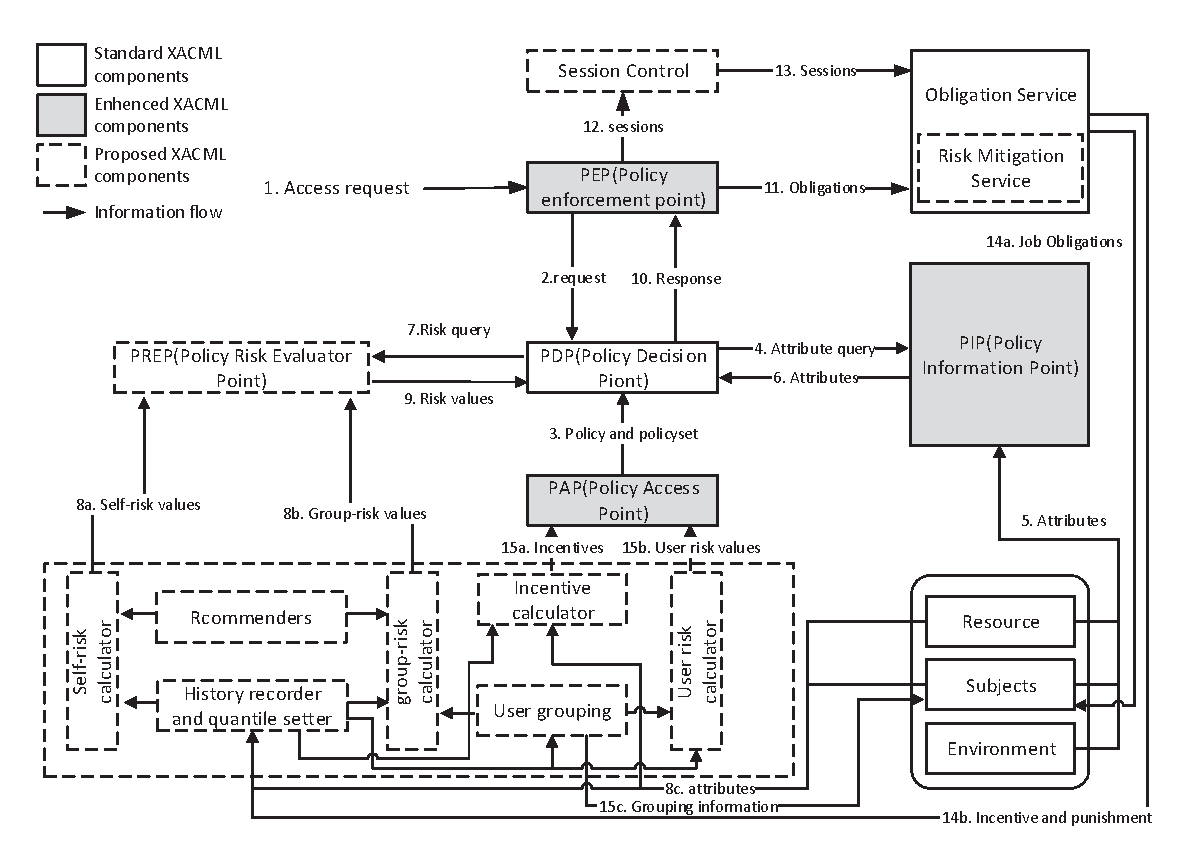
\includegraphics[width=\linewidth]{./figures/Process_flow.eps}
	\label{fig:Process_flow}
	\caption{基于XACML的风险自适应访问控制模型处理流程}
\end{figure*}

对于XACML的标准框架,一旦策略决策点 (PDP) 收到了来自请求者 (即访问控制系统的用户,即访问主体) 的访问请求, 它首先会从策略访问点 (PAP) 和策略信息点 (PIP) 然后决定接受还是拒绝该请求。 此外,策略执行点 (PEP) 难以处理与请求者的交互,策略访问点 (PAP) 是静态的,并且义务服务和策略信息点 (PIP) 都缺乏风险管理。
在我们提出的方法中,对PEP,PIP和PAP进行了增强,并添加了新的三个组件,即策略风险评估器点 (PREP),会话控制和风险缓解服务 (嵌入在义务服务的组件中) 然后,一旦PDP收到来自经过身份验证的用户的访问请求,并且在做出决定之前,它会请求与指定主题 (即下划线用户) 和历史访问记录相关的风险值。 此外,在做出决定后,一些反馈信息将提供给义务服务。 所提出的风险自适应访问控制模型的流程如图\ref{fig:Process_flow}所示。 该框架是基于标准可扩展访问控制标记语言 (XACML) 提出的,与 \cite{shaikh2012dynamic}的框架有所不同。 我们方法中的所有新组件均以虚线突出显示,所有增强的组件均以浅灰色突出显示。

在基于标准XACML的新框架中,所有访问请求均由经过身份验证的用户发送,我们称此类用户为主题。 从步骤1到步骤6,该过程类似于Shaikh等人\cite{shaikh2012dynamic} 和Verma \cite{verma2004xml}的过程。  一旦收到所有必需的信息,PDP就将有关当前请求的风险查询发送到PREP (步骤 7). PREP根据用户的过去行为和历史行为的风险值来评估风险值 (步骤 8). 每个请求都有两个风险值,一个是根据下划线用户自己的过去行为评估的自我风险值,另一个是根据所有用户的过去行为以及所有用户评估的群体风险值与下划线用户属于同一组。
如果系统没有足够的历史记录,则PREP将根据建议评估两个值。与特定请求相关的当前风险值将返回到PDP (步骤 9). 根据风险值,PDP做出决定。将此决定转发给PEP,由其执行 (步骤10). 无论是允许访问还是拒绝访问,PEP都会通知 (步骤 11) 义务服务,该服务将决定是否需要风险缓解服务。在强制执行的延迟时间内,会话控制组件监视请求者的行为,并管理访问会话 (步骤 12). 如果在该会话中访问行为的风险太高,则会话控制通知义务服务组件并控制该会话中的请求 (例如,终止会话) (步骤 13). 义务服务将决定是激励还是惩罚用户,并更新主体的属性 (例如工作义务) (步骤 14). PREP定期通过激励机制重新分配预算配额,重新将用户标识为正常用户或有风险的用户,并将用户识别为更合适的组 (步骤 15).

\subsection{请求风险值和请求决策}
\label{subsec:risk values and decision}
\subsubsection{请求风险值}
我们动态评估访问请求风险值的方法是根据请求者的过去行为以及基础请求者所属组的所有成员而设计的。对于特定的用户组,该组中的每个人都按照相似的工作职责分组到该组中,并且工作职责在一段时间内相对稳定,并且会在很长一段时间内自然演变。对于指定的用户,他所属的组可能会随时间改变。因此,应该根据用户本人和组的时间短来评估特定组中用户的访问请求,可以根据用户本人和组的时间长来识别用户。在本节中,我们仅关注对特定用户的请求的评估。直观地,如果一段时间内没有访问该请求的预期信息,即使这些信息可能长时间访问,该请求的风险值也将很高。我们将这种想法应用于评估访问请求的风险。
受Shannon \cite{shannon1948mathematical} 启发的信息理论在衡量信息价值方面非常有效。我们采用了一些信息理论的概念,并对它们进行了改进,以设计自己的风险评估功能。

令 $u \in U$ 是已认证用户集 $U$, 并且 $u$ 属于用户组 $g$ ,该用户组$g$ 是 $U$ 的子集. $u$ 的请求 $q$ 有一定的风险,表示为 \emph{自风险} $sr$ 和 \emph{组风险} $gr$ ,已在定义 \ref{def_self_risky} 和 \ref{def_group_risky} 中提出.


令 $(q_1, q_2, ... , q_{n-2}, q_{n-1})$ 为 $u$ 的 $n-1$ 倍允许请求,而 ${r_1, r_2, ... , r_{n-2}, r_{n-1}}$ 分别为这些请求的访问记录集。 令 $q_n$ 是用户当前的访问请求, 预期的记录集为 $r_n$. 如果我们将每对 $(q_n,r_n)$ 视为随机事件,则该对 $(q_i,r_i)$ 的信息量可以通过\textbf{自信息}表示。那么当前访问请求的 $sr$ 可以解释为

\begin{equation}
\label{eq:self risk}
sr(u,q_n)=I(q_n,r_n)
\end{equation}

在等式 \ref{eq:self risk} 中, 我们可以从 $r_n$ 中预期记录的概率得出 $rs$ . 并且不同的记录集可能具有相同的敏感信息,因为它们具有相同的标签。 因此,在不同的情况下应使用不同的分类。 可以将关系数据库中的记录分类为相同的记录,以使这些记录具有相同的信息,并且在电子医疗系统中,具有相同信息的医疗记录应按标签分类 (例如ICD-9或 ICD-10代码).

为方便起见,我们将访问请求 $q$ 和预期记录集 $r$ 视为相同, 即,每个不同的访问请求都打算使用具有不同信息的不同记录。 假设访问请求集 $Q_u$ 中有 $k$ 个不同的请求 $q_1,q_1,....,q_k$ ,其中包括过去的 $n-1$ 次访问请求和的 $u$ 的当前访问请求 $q_n$ ,以及概率分别为 $p_1,p_2,...,p_k$ . 如果在 $k$ 个不同的请求中 $q_n$ 与 $q_i$ 相同,则方程 \ref{eq:self risk} 可以简化为

\begin{equation}
\label{eq:self risk 2}
sr(u,q_n)=I(q_i)=-logp_i
\end{equation}

公式 \ref{eq:self risk} 和 \ref{eq:self risk 2} 都在有足够的历史记录供 $u$ 使用的条件下,如果没有足够的历史记录供 $u$ 访问, 我们可以使用默认值 (例如1) 或整个历史记录。
\begin{small}
	\begin{equation}
	\label{eq:self risk 3}
	sr(u,q_n)=
	\left\{
	\begin{array}{ll}
	I(q_i)=-logp_i, & \hbox{是否有足够的历史记录;} \\
	Avg(I(u,q)), & \hbox{如果历史还不够;} \\
	1, & \hbox{如果没有可用的历史记录。}
	\end{array}
	\right.
	\end{equation}
\end{small}

$rs$ 的计算基于 $u$ 自己过去 $n-1$ 次访问行为的马尔可夫链。并且马尔科夫链的长度可以根据需要针对每个用户进行动态和个性化设置,然后我们可以适当地平衡用户 $u$ 的近期历史和长期历史行为。

令 $sr(u, q_1), sr(u, q_2), ... , sr(u, q_{n-2}), sr(u, q_{n-1})$ 为过去 $n-1$ 次允许请求 $u$ 的自风险值,并令 $sr(u,q)$ 为 $u$ 当前 (第n次) 请求 $q$ 的当前自风险值. 令 $\epsilon_s \in (0,1)$ 为分位数。 通过定义 \ref{def_self_risky} 可以轻松地将 $q$ 定义为 \textbf{自风险请求} 或 \textbf{自正常请求} 。

类似地,可以通过该马尔可夫方法获得下位用户 $u$ 的当前访问请求的组风险值。 令 $q_1,q_1,....,q_l$ 是访问请求集 $Q_g$ 中的元素,它表示组 $g$ 过去的 $m-1$ 次允许访问请求和 $u\in g$ 的当前访问请求 $q_m$, $p_1,p_2,...,p_l$ 分别为概率。 如果 $q_m$ 与 $Q_g$ 中的 $q_i$ 相同, 则 $gr(g,q_m)$ 可被计算为
\begin{small}
	\begin{equation}
	\label{eq:group risk}
	sr(g,q_m)=
	\left\{
	\begin{array}{ll}
	I(q_i)=-logp_i, & \hbox{如果有足够的历史记录 ;} \\
	Avg(I(g,q)), & \hbox{如果历史还不够;} \\
	1, & \hbox{如果没有可用的历史记录。}
	\end{array}
	\right.
	\end{equation}
\end{small}
并且,我们可以通过定义 \ref{def_group_risky} 将 $u\in g$ 的访问请求 $q$ 识别为 \textbf{组风险请求}   \textbf{组正常请求} 。


\subsubsection{Decisions}
自风险值 $sr(u,q)$ 和组风险值 $gr(g,q)$ 都是访问决策的基础。 作为定义 \ref{def_self_risky} 和 \ref{def_group_risky}, 我们可以将所有用户的请求分为四类,这意味着访问请求 $q$ 有四个不同的风险级别。然后,我们可以根据请求的风险级别做出决策,如下所示。
\begin{footnotesize}
	\begin{equation}
	\label{eq:decision}
	decision=
	\left\{
	\begin{array}{ll}
	p, & \hbox{if $q$ is a self and  a group normal request;} \\
	p(rm), & \hbox{if $q$ is a self risky and a group normal request;} \\
	d, & \hbox{if $q$ is a self and a group risky request;} \\
	d(p), & \hbox{if $q$ is a self normal and a group risky request.} \\
	\end{array}
	\right.
	\end{equation}
\end{footnotesize}
如果 $p$ 表示请求是正常的并且没有风险,则 $p(rm)$ 表示风险较低,因此可以降低风险,并且应在用户采取一定风险缓解措施后确保其进入。 $d$ 表示当风险高时则拒绝 , $d(p)$ 表示风险太高,应限制用户使用。

等式 \ref{eq:decision} 的决定基于以下原因。 如果请求既是自身正常请求又是组正常请求,则用户和组在过去一段时间内频繁访问预期记录,因此该请求是正常的而且没有风险。 如果某个请求是自风险请求,并且是组正常请求,则表示该组中的其他用户(非用户本人)经常访问了预期记录,这些记录与该组的工作职责相关,但用户几乎不访问,并且对该用户的访问风险很小,应该在系统采取某些适当的风险缓解措施后授予访问权限。如果某个请求是自风险请求,并且是组风险请求,那么该组几乎不会访问预期记录,这些记录与该组的工作义务无关,因此访问请求应被拒绝。如果某请求是一个自正常请求,并且是一个组风险请求,那么该组几乎不会访问预期记录,并且这些记录与该组的工作职责无关,但该用户已多次访问记录,因此应拒绝访问此请求,并要加重处罚。
\subsection{用户分类与激励机制}
\label{subsec:User classification and incentive mechanism}
在本节中,我们首先介绍根据用户 $u$ 和组 $g$ 的历史访问请求,定期将用户 $u \in g$ 识别为好奇用户还是诚实用户的方法。然后提出用户如何定期从一个组迁移到另一个组的方式; 最后设计了一种监督访问行为,抑制风险请求和风险用户的激励机制。所有这些方法都与马尔可夫模型相似,也是基于信息论的。

\subsubsection{用户的风险值和用户分类}
对于指定用户组中的用户,我们可以在假设 \ref{ass:user_obligations} 和 \ref{ass:honest_user} 下通过定义 \ref{def_curious user} 将用户识别为好奇用户还是诚实用户。  但实际上很难找到 $\theta_g$ 的特定函数。 在我们的方法中,我们通过使用组 $g$ 的访问模式来近似函数 $\theta_g$ 。信息熵可以用来表示信息集的不确定性,我们采用香农熵来表示组和用户的访问模式。 用户熵越高,用户越好奇。

令 $T$ 为周期时间, $Q_{g,T}=(q_1, q_2,...,q_{s_g})$ 为 $T$ 中 $u$ 组所有用户的访问请求, $Q_{g,T}$ 遵循分布
$P(g,T)=
(
\begin{array}{l}
q_{g,1},  q_{g,2}, ...,q_{g,n_g}\\
p_{g,1},  p_{g,2}, ...,p_{g,n_g}\\
\end{array}
)
$.
令 $Q_{u,T}=(q_1, q_2,...,q_{s_u})$ 为 $T$ 中来自用户 $u \in g$ 的访问请求, $Q_{u,T}$ 遵循分布
$P(u,T)=
(
\begin{array}{l}
q_{u,1},  q_{u,2}, ...,q_{u,n_u}\\
p_{u,1},  p_{u,2}, ...,p_{u,n_u}\\
\end{array}
)
$.

然后可以计算出用户 $u \in g$ 在时间段 $T$ 中的风险值 $risk(u,T)$ 为


\begin{equation}\label{eq:user risk}
risk(u,T)=max \{\frac{H(P(u,T))-H(P(g,T))}{H(P(g,T))},0\}
\end{equation}

等式 \ref{eq:user risk} 表示在过去的时间段 $T$ 中,用户风险随熵的增加而线性增加。但实际上,始终存在阈值 $\phi$, 使得用户A和用户B的风险相似, 当 $H(P(A,T))>H(P(B,T))>\phi$ 时,甚至 $H(P(A,T))-H(P(B,T))$ 非常大。然后可以将公式 \ref{eq:user risk} 中的风险值提高为

\begin{equation}\label{eq:user risk 2}
risk'(u,T)=\alpha ^ {max \{H(P(u,T))-H(P(g,T)),0\}}
\end{equation}

其中 $\alpha \in (0,1)$, 而风险的结果 $risk'(u,T)$ 将是 $[\alpha, 1)$ 中的实数。 等式 \ref{eq:user risk 2} 中陈述的函数是平滑的,并且实际上更合适。

因此,一个用户 $u \in g$ 可以由过去一段时间 $T$中的风险值 $risk(u,T)$ 或 $risk'(u,T)$ 来标识。 如果 $risk(u,T) > 0$ 或 $risk'(u,T)>\alpha$, 我们称 $u$ 在过去一段时间 $T$ 中是好奇用户, 我们称 $u$ 为诚实用户,前提是  $risk(u,T) = 0$ or $risk'(u,T)=\alpha$. 形式上,

\begin{equation}\label{eq:user type}
type(u,T)=
\left\{
\begin{array}{ll}
c, & \hbox{iff $risk(u,T) > 0$ or $risk'(u,T)>\alpha$;} \\
h, & \hbox{iff  $risk(u,T) = 0$ or $risk'(u,T)=\alpha$.} \\
\end{array}
\right.
\end{equation}

公式~\ref{eq:user type} 为一段时间内的用户分类提供了基础, 但是我们并不总是在短时间内将一个人分类为好人还是坏人。 实际上,在某些情况下我们需要对一个人进行长时间的调查,这里我们对用户 $u \in g$ 的风险值进行多次评估,然后形成 $u$ 的风险值链。设 $T_n$ 为当前期间,$T_0, T_1, T_2, ..., T_{n-1}$ 为过去 $n$ 个时期,$n$ 个时期 $u \in g$ 的用户风险值可分别通过 $risk(u,T_0),risk(u,T_1),risk(u,T_2),..., risk(u,T_{n-1})$ (or $risk'(u,T_0), risk'(u,T_1), risk'(u,T_2), ..., risk'(u,T_{n-1})$)给予。因此,我们可以根据过去的 $n$ 个风险值 $u$ 来确定当前期间的用户,如下所示

\begin{equation}\label{eq:user type Tn 1}
type(u,T(n))=
\left\{
\begin{array}{ll}
c, & \hbox{if $conut(risk(u,T_i) > 0) > n/2$;} \\
h, & \hbox{if $conut(risk(u,T_i) > 0) \leq n/2$.} \\
\end{array}
\right.
\end{equation}
而且
\begin{equation}\label{eq:user type Tn 2}
type(u,T(n))=
\left\{
\begin{array}{ll}
c, & \hbox{if $conut(risk'(u,T_i) > 0) > \alpha$;} \\
h, & \hbox{if $conut(risk'(u,T_i) > 0) \leq \alpha$.} \\
\end{array}
\right.
\end{equation}

如果 $u$ 在过去 $n$ 个周期中始终是一个好奇用户,我们称 $u \in g$ 在过去 $n$ 个周期中是一个好奇用户,否则,他是一个诚实的用户。

\subsubsection{组中的用户迁移}
组织中的成员具有不同的工作职责,可以按相似的职责将其分组。 随着时间的变化,指定成员可能会随着其义务的改变而从A组迁移到B组,并且新义务比A组更接近B组中的用户。对于我们的访问控制模型的用户, 他们可以随着工作职责的变化而在小组中迁移,并且我们通过观察访问行为定期将指定的用户分类为最合适的小组。

首先,我们定义指定用户和用户组之间的距离。 直观地,对于用户和组的工作义务,义务越相似,距离就越近。 特别是,如果指定用户的工作义务与组(即该用户是该组的成员)的工作义务相同,则距离为零。从访问行为模式的角度来看,对于诚实用户而言,如果该用户在最合适的组中被识别,则不会存在访问风险,否则,即使他是诚实用户也始终具有正风险值。

\begin{definition}%[user-group distance]
	\label{user-group distance}
	设 $T$ 为周期时间, $u$ 为用户 , $g$ 为一个组. 假设 $u$ 是 $g$ 的成员,则 $t$ 中 $g$ 的风险值 $risk(u,T)$ 或 $'risk(u,T)$ 可以通过公式 \ref{eq:user risk} 和 \ref{eq:user risk 2}, 则我们称 $d(u,g,T)=risk(u,T)$ or $d(u,g,T)=risk'(u,T)$ 是 $T$ 中 $u$ 和 $g$ 的 \textbf{距离} 。
\end{definition}

为方便起见,我们仅讨论 $risk(u,T)$ 的公式。

\begin{claim}用户组距离]
	如果 $u$ 是诚实用户,并且 $g$ 是时段 $T$ 中 最适合 $u$ 的组, 则 $d(u,g,T)=0$ (或如果采用 $risk'$ ,则$d(u,g,T)=\alpha$ ).
\end{claim}

\begin{claim}
	如果 $u$ 是诚实用户,并且我们观察到在时间段 $T$ 中的访问行为。那么总存在一个组 $g \in G$ ,使得 $d(u,g,T)=0$.
\end{claim}

在识别用户是否已迁移之前,我们应该观察访问行为数次,原因是由于行为是连续的,因此用户迁移过程很慢。 如果指定的用户正在迁移,则必须连续增加用户的风险,这意味着当前组不适合他,或者他确实是好奇用户 (在这种情况下,对他的惩罚是严重的,请参阅第 \ref{subsec:Incentive mechanism}节 )。 然后,我们如下定义迁移的用户。

\begin{definition}%[user-group distance]
	\label{def:migrating user}
	设 $T_0,T_1,...,T_{n-1}$ 为过去的 $n$ 个周期, 而 $risk(u,T_0),risk(u,T_1),risk(u,T_2),..., risk(u,T_{n-1})$ 分别为 $n$ 个时期 $u\in g$ 的用户风险值。 如果存在周期 $T_i$ 使得 $risk(u,T_0) = risk(u,T_1) = ... = risk(u,T_{i-1}) =0  < risk(u,T_{i}) \leq risk(u,T_{i+1}) \leq ... \leq risk(u,T_{n-1})$, 那我们称 $u$ 是一个 \textbf{迁移用户}.
\end{definition}

注意 "$\leq$"的关系 "=" 不能全部成立。我们应该重新认识正在迁移的用户,使其成为最合适的组。与诚实用户 $u$ 从 $g$ 迁移相反,如果 $g'$ 是目标组,则 $u$ 与 $g'$ 之间的距离会越来越近,直到为零。

\begin{definition}%[user-group distance]
	\label{def:target group}
	设 $T_0,T_1,...,T_{n-1}$ 为过去的 $n$ 个周期,$u \in g$ 为迁移用户。如果存在 $g' \in G/g$ 使得 $d(u,g,T_0) = d(u,g,T_1) = ... = d(u,g,T_i) \geq d(u,g,T_{i+1}) \geq ... \geq d(u,g,T_{n-1}) = 0$, 那么称 $g'$ 为当前周期 $u$ 的 \textbf{目标组} 。 
\end{definition}

如果可以找到 $u$ 的目标组 $g'$ ,则我们将 $u$ 识别为新组,并用 $g'$ 更改 $u$ 的组信息,否则,我们将采用第 \ref{subsec:Incentive mechanism} 节中介绍的激励机制,并不断观察访问行为。

\subsubsection{Incentive mechanism}
\label{subsec:Incentive mechanism}

在银行的信用体系中,初始信用额是一个对普通消费者来说足够的常数。 一旦某人获得了初始信用卡,银行就会评估该指定人的每一种消费行为,确定该消费行为是否违法,并拒绝该违法行为; 在每个周期 (例如一个月或六个月), 银行都会识别此人是否有风险,并根据该时间段内他的行为适当调整其下一个期间的信用额度; 有时,银行会通过长期观察信贷行为来识别人,例如五年。受信贷系统概念的启发,我们在本节中为风险自适应访问控制系统提出一种访问控制激励机制。

\textbf{初始化} 不同组的初始风险配额不同,并且初始风险配额将被初始化为访问控制系统中的每个风险配额。 另外,初始风险配额将由用户在请求访问时消耗,并且初始风险配额对于一段时间内的诚实用户而言已足够。 我们将 $u \in g$ 指定为 $g$ 组的用户,$g$ 的初始风险配额为 $qt_{g,init}$ (这意味着组 $g$ 中包括 $u$ 的每个人都具有相同的 $qt_{g,init}$)。 $g$ 的新用户将由相同的 $qt_{g,init}$ 初始化,风险配额将根据 $u$ 的历史访问行为在新的时间段内重新分配给 $u$ 。 注意,一旦访问控制系统被初始化,组 $g$ 的初始风险配额就可以随着 $g$ 的工作义务的发展而改变。

\textbf{消耗量} 在一段时间内,每个访问请求将消耗一定数量的 $qt_{g,init}$ 。风险配额将在下一个时期重新分配。风险配额消耗的增加取决于访问请求的决定。正如我们在第 \ref{subsec:risk values and decision}节中所述,访问请求有4种不同的决策类型,因此有4种减少访问消耗的数量类型。 令 $q$ 为周期 $T$ 中对 $u \in g$ 的访问请求。 如果决策 $decision(q)=p$ ,则风险消耗量为$c_p$ ;如果决策 $decision(q)=p(rm)$ 且风险缓解措施确定为 $q$ ,则风险消耗量为$c_p$ 。如果决策 $decision(q)=p(rm)$ ,而没有风险缓解措施 $q$ ,则风险消耗量为 $c_{p(rm)}$ ;如果决策 $decision(q)=d$ ,则风险消耗量为 $c_d$ ; 如果决策 $decision(q)=d(p)$ ,则风险消耗量为 $c_{d(p)}$ ;其中 $c_p <= c_{p(rm)} < c_d < c_{d(p)}$. 如果在时段 $T$ 中 $u$ 的请求正常,则 $u$ 的风险配额将始终减少到接近零的正数,并且如果 $T$ 中拒绝了 $u$ 的某些访问请求,则必须将风险配额减少到零。拒绝的请求越多,风险配额用尽的时间就越早。

\textbf{风险配额重新分配} 对于新的时间段,应该根据过去时间段内的访问行为重新分配组 $g$ 中每个用户的风险配额。 在这里,我们提出了三种风险配额重新分配方法,一种基于最后一个时期,一种基于最后一个时期和过去 $n$ 个时期,第三种是前两个时期的组合。

\begin{itemize}
	\item \textbf{单周期方法} 设 $u \in g$ 为 $g$ 组的用户,当前时期为 $T$, 该时期 $u$ 的风险份额为 $qt_{u,T}$ 。 设 $qt_{u,T'}$ 是 $u$ 在最后一个时期 $T'$ 的风险配额。
	然后根据等式 \ref{eq:user risk} 和 \ref{eq:user type}, 我们得到
	\begin{small}
		\begin{equation}\label{eq:risk quota re-allocation 1}
		qt_{u,T}=
		\left\{
		\begin{array}{ll}
		qt_{g,init}, & \hbox{if $type(u,T')=h$;} \\
		qt_{u,T'}\cdot (1-risk(u,T')), & \hbox{if $type(u,T')=c$.} \\
		\end{array}
		\right.
		\end{equation}
	\end{small}
	而且,我们可以基于方程式 \ref{eq:user risk 2} 和 \ref{eq:user type} 轻松获得方程式 \ref{eq:risk quota re-allocation 1} 的替代方程式。
	\item \textbf{多周期方法} 令 $T_0,T_1,...,T_{n-1}$ 为过去的 $n$ 个周期,而 $risk(u,T_0),risk(u,T_1),risk(u,T_2),..., \\risk(u,T_{n-1})$ 分别为 $n$ 个周期内 $u$ 的用户风险值。 因此 $T'$ 与 $T_{n-1}$ 相同,而 $risk(u,T')$ 与 $risk(u,T_{n-1})$ 相同。 $u \in g$ 的新风险定额可以通过以下公式获得
	
	\begin{footnotesize}
		\begin{equation}\label{eq:risk quota re-allocation 2}
		qt_{u,T}=
		\left\{
		\begin{array}{ll}
		qt_{g,init}, & \hbox{if $type(u,T(n))=h$;} \\
		qt_{u,T'}\cdot (1-\frac{ \sum _{i=0} ^ {n-1}risk(u,T_i))}{n}), & \hbox{if $type(u,T(n))=c$.} \\
		\end{array}
		\right.
		\end{equation}
	\end{footnotesize}
	
	\item \textbf{组合方法} 有时,我们应该权衡近期历史和长期历史。将\textbf{单周期方法}和\textbf{多周期方法}相结合的加权方法非常有效。设 $\omega_1, \omega_2 \in (0,1)$ 且 $\omega_1+ \omega_2 =1$, 则可计算出当前周期 $T$ 的风险配额 $qt_{u,T}$ 
	\begin{equation}\label{eq:risk quota re-allocation 3}
	\begin{aligned}
	qt_{u,T} &= qt_{u,T'}\cdot (\omega_1(1-\frac{ \sum _{i=0} ^ {n-1}risk(u,T_i))}{n}) \\
	&+ \omega_2(1-risk(u,T')))
	\end{aligned}
	\end{equation}
\end{itemize}

可以将上述三种方法中的用户风险值 $risk(\cdot,\cdot)$ 替换为公式 \ref{eq:user risk 2} 中指定的 $risk'(\cdot,\cdot)$ 。

\subsection{其他改进的组件}
\label{subsec:Other improved components}
如第 \ref{subsec:framework} 节中的图\ref{fig:Process_flow} 所示,与标准XACML相比,我们的风险自适应访问控制模型中包含三个新组件和三个增强组件。PREP的详细信息已在 \ref{subsec:risk values and decision} 和 \ref{subsec:User classification and incentive mechanism}节中讨论,其他组件将在本节中讨论。

\textbf{会话控制} 在此会话控制组件中,通过执行时间的属性来管理策略执行点阶段的应用。 策略的执行并非总是实时的 (例如,下载文件或调用程序来完成某些任务), 然后可以量化此会话中的访问行为所造成的损害。 因此,会话会监视当前会话中发生的这些损害,以确保策略允许风险级别。 一旦损坏发生超出允许的风险范围,访问会话将被访问控制系统挂断或中断。

\textbf{减轻风险服务} 风险缓解服务是义务服务中添加的组件,它提供了一些缓解风险的措施。 该组件有助于访问控制系统降低访问请求的风险。 PDP需要降低风险的服务后,将验证一些其他增强安全性的措施 (例如,审核,认证) 。

\textbf{政策执行点} 通过一些新的附加功能,增强了策略执行点,例如添加了会话模型。 这样,PEP就可以与外部应用程序和义务服务组件进行交互,从而方便地管理外部应用程序的状态并降低访问请求的风险。

\textbf{点接入点} 我们会根据用户的风险值为PAP提供动态访问策略模型。 这些策略将定期重置或调整。

\textbf{政策信息点} 增强的PIP中还有更多属性,这些属性对于风险量化很有用。 例如,除了时间,位置和访问度量外,还添加了风险配额,分组信息等。

\section{讨论与分析}
\label{sec:Discussion and analysis}
由于传统的访问控制系统不是基于风险的,因此,我们仅讨论分析,并与本节中的相关工作进行比较。

大量增加基于风险的工作流程的访问控制,其中大部分集中在将风险纳入多级安全性的建议方法 \cite{cheng2007fuzzy,ni2010risk} 和角色 \cite{chen2011risk,choi2015framework}。 但是,基于云的大规模信息系统中潜在的安全性和隐私要求趋向于适应风险意识的访问控制模型,例如 \cite{wang2011quantified,shaikh2012dynamic,khambhammettu2013framework} 中所述。

首先,我们的工作实施起来非常方便。 这项工作通过一些新的增强组件扩展了XACML标准,以支持风险自适应访问控制。Chen and Jason 等人 \cite{Chen2013} 争论了如何将XACML标准扩展到基于风险的访问控制中, \cite{santos2014dynamic} 的最新工作表明XACML描述的基于风险的访问控制在云环境中是可实现的和有效的。相对地,我们实施风险自适应访问控制的方法完全符合XACML标准,而无需引入额外的元素。 因此,我们的模型和 Shaikh 等人 \cite{shaikh2012dynamic} 是现实生活中可以实现的。

其次,我们的方法对于现实生活中的场景更为实用。风险评估是风险基础访问控制系统的核心,所有现有工作 \cite{wang2011quantified, shaikh2012dynamic, khambhammettu2013framework} 通过使用 "threat(subject, object)-impact(object, action)", "trust-threat", "trust level-risk level" 来量化访问请求或访问行为的风险值。管理员必须使用相同的方法对主题和对象 (有时甚至是目的和动作) 进行分类,而这种方法很难设计或发现。此外,这些工作中的风险评估过程有些主观。在我们的工作中,仅访问对象才需要特定类别,可以通过标记或标记轻松实现。无需识别特定主题的特定角色或工作义务,访问控制系统可以识别特定组中的用户所承担的某些义务与该组中其他用户的义务相似,而无需专门知道 什么是工作义务。实际上,我们的方法更容易计算访问请求和用户的风险值。

第三,在我们的工作中对访问请求和用户的标识更加精确。 几乎现有的工作 (例如 \cite{wang2011quantified,shaikh2012dynamic}) 会评估用户或请求的风险值,然后根据历史访问行为对请求做出决策并识别用户。 除了Shaiare更精确的要求和用户的风险值外,所有这些工作都没有考虑到近期历史和悠久历史之间的平衡,所有这些风险值都是通过准马尔可夫模型计算的。这些值平衡了最近的访问/请求历史记录和长时间的访问/请求历史记录。 然后,通过将当前访问请求与用户自身及其所属组的访问历史进行比较,基于前两个风险值做出决策。 通过将一个用户的访问/请求模式与其所属的组的访问/请求模式进行比较,基于第三类风险值识别用户。 这样,决策就变得更加合理,识别也更加精确。

第四,我们的激励机制更加有效。 除 Shaikh, Adi 和 Logrippo \cite{shaikh2012dynamic}外,相关工作中未考虑任何激励机制。 \cite{shaikh2012dynamic} 作者提出了一种以电子现金支付为灵感的“奖罚”方法,但并未描述通用机制。 在我们的工作中,提出了一种类似于信用体系的精细激励机制。 风险配额是根据用户的请求和访问行为定期分配给用户的。 如果根据过去或过去一段时间的历史行为将其识别为好奇的用户,则其激励机制将降低其风险配额; 如果特定用户的一个请求被确定为有风险,则风险配额将被消耗得多。访问请求的风险越大,则风险配额将被消耗的越多。然后,我们的激励机制可用于监督访问请求和 用户,并限制有风险的请求和好奇的用户。

\section{小结}
\label{sec:Conclusion}
传统信息系统中使用的访问控制模型根据固定的预定策略来决定是否允许访问。 这些策略始终很难执行,并且没有考虑系统中访问行为的动态管理。令人担忧的是,使用此模型,通常会授予对不必要信息的访问权限,并且未遵守“需要知道”的原则。 因此,由于传统访问控制模型的自然缺陷,在这种系统中出现了很多敏感数据和隐私泄露的情况。

在本文中,我们提出了一种准-马尔科夫风险自适应访问控制方法,该方法提供动态访问控制,以便在访问信息系统中的记录或信息时仅提供用户工作义务所需的信息。 在我们的方法中,设计了一个基于标准XACML的修改框架,定义了三个附加组件,并增强了标准XACML框架的三个组件。 为了考虑用户在访问控制系统中的访问请求风险,根据工作职责将所有用户分为不同的非相交组。 通过将请求与用户和组的历史访问行为进行比较,可以计算出对特定用户组中用户的访问请求的风险值。此外,我们通过基于马尔可夫的方法定期地将用户识别为诚实用户或好奇用户,并且该方法可以权衡近期历史和悠久历史的权重。 最后,提出了一种基于信用体系的激励机制,监督所有用户履行其工作职责。所提出的访问控制模型对于基于云的庞大信息系统非常有效,因为所有策略,访问请求风险值 (历史记录的长度), 用户标识 (历史记录的周期), 以及激励措施都是自适应的。  而且,我们只需要标记存储的数据 (对象) 而无需标记用户 (主题) 或信任计算。

将来,我们将探索基于信誉的激励机制,并将其应用于基于风险的访问控制系统中。 此外,基于理性风险的混合访问控制系统对研究也非常有价值。